%\documentclass[10pt]{beamer}
\documentclass[xcolor={pdftex,dvipsnames,table}]{beamer}

\definecolor{redUnipd}{HTML}{9b0014}
\definecolor{grayUnipd}{HTML}{444F51}
\definecolor{myblue}{HTML}{317a9b}
%\definecolor{Black}{RGB}{0,62,114}
\newcommand{\bbf}[1]{\textcolor{black}{\bf #1}}
\newcommand{\rbf}[1]{\textcolor{redUnipd}{ #1}}
\usefonttheme{structurebold}
\usecolortheme[named=myblue]{structure}
\setbeamercolor{structure}{fg=redUnipd}
\setbeamercolor{normal text}{bg=white,fg=grayUnipd}
\setbeamertemplate{itemize items}{$\circ$}
%\textopenbullet
%\usepackage{marvosym}
%\setbeamertemplate{itemize items}{$\Neutral$}

\usepackage{pgfpages}
\pgfpagesuselayout{resize to}[a4paper, 
                                border shrink=1.5cm,
                                landscape]

\usepackage[T1]{fontenc}
%
\usepackage[english]{babel}
\usepackage{graphicx}
\usepackage{booktabs}
\usepackage{latexsym}
\usepackage{subfigure}
\usefonttheme{professionalfonts}
%\usepackage{enumitem}
\usepackage{amsmath,amssymb}
\usepackage[latin1]{inputenc}
%\setbeamercovered{dynamic}
\usepackage{Sweave}
\usepackage[english]{babel}
\usepackage{tikz,comment,amssymb}
\usetikzlibrary{shapes}

\newcommand{\bb}[1]{\begin{block}{#1}}
\newcommand{\eb}{\end{block}}
\newcommand{\bi}{\begin {itemize}}
\newcommand{\ei}{\end{itemize}}
\newcommand{\be}{\begin {enumerate}}
\newcommand{\ee}{\end{enumerate}}
\linespread{1.05}

\newcommand{\bfr}[1]{\begin{frame} \frametitle{#1}}

\AtBeginSection[] {
  \begin{frame}<beamer>
    \frametitle{Outline}
    \tableofcontents[currentsection]
  \end{frame}
}


\title[]{Controllo della Molteplicit\`a nei trial clinici}
\subtitle{Biostatistica avanzata per la ricerca clinica}
\author[\hspace{5cm}]{Livio Finos}
\date{}
% \date{A.A. 2015/2016 }
%\logo{
\includegraphics[scale=.05]{figures/logoUnipd.jpg}}

\begin{document}

\begin{frame}
  \titlepage
\end{frame}


\section{Introduzione}

% \section{Alcuni Esempi}

\bfr{Microarray study}
  \bb{Top 5 genes out of 20000}
    {\scriptsize\begin{tabular}{lrr}
    Gene & p-value  \\ \hline
  OCIAD2 &5.5e-6  \\
    NEK3 &6.7e-6  \\
    TAF5 &7.1e-6  \\
 FOXD4L6 &7.5e-6  \\
    ADIG &8.8e-6  \\
  \textbf{\vdots} & \textbf{\vdots} \\\hline
  \end{tabular}}
  \eb
  \bb{Small p-value?}
    \bi
      \item un p-value di 5.5e-6 \`e improbabile (evidenza per $H_1$)
      \item ma \`e improbabile anche se consideriamo di averlo cercato tra 20000 test?
      \item Possiamo veramente dire che OCIAD2 \`e differentially expressed?
      \item e a proposito di NEK3?
    \ei
  \eb
\end{frame}


%%%%%%%%%%%%%%%%%test multipli
%\subsection{Quando test multipli?}
\bfr{Ulteriore Esempio: studi fMRI}

\begin{columns}
\column{0.5\textwidth}
 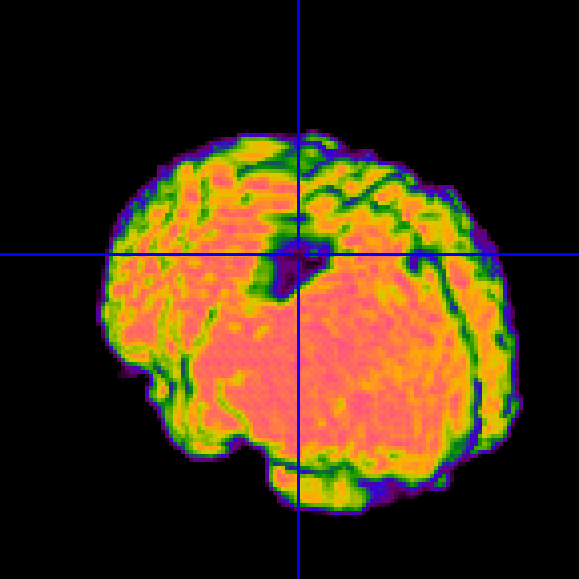
\includegraphics[scale=.5]{plaatjes/fMRI.png}
\column{0.5\textwidth}
Una mappa di attivit\`a celebrale per ogni soggetto\\ \pause
Ogni voxel (punto) produce un p-value\\ \pause
L'output \`e solitamente una lista dei voxel pi\`u attivi \\ (sui migliaia testati)
\end{columns}
\textcolor{redUnipd}{\textbf{Dubbio}}: necessario controllo della molteplicit\`a?

\end{frame}

\bfr{Altri esempi, pi\`u frequenti}
  \bb{Modelli di Regressione (LM e GLM)}
    Un t-test per ogni Coefficiente di Regressione
  \eb
  \bb{Anova}
    Tutti i Confronti a Coppie (post-hoc)
  \eb
\bb{Ogni volta in cui l'analisi produce pi\`u di un p-value}
\eb
\textcolor{redUnipd}{\textbf{Dubbio}}: necessario controllo della molteplicit\`a?
\end{frame}


\bfr{\ldots e a proposito di trial clinici:}
  \bb{Multiple endpoints}
  es: pi\`u endpoints sono importanti per valutare la guarigione del paziente
\eb
  \bb{Multiple doses}
    es: Placebo vs Dosi crescenti\\ vogliamo i Confronti a Coppie (post-hoc)
  \eb
\bb{Multiple sub-groups}
es: la terapia funziona solo su sottogruppi della popolazione, \\
ad esempio con un preciso corredo genetico
le donne
\eb
\textcolor{redUnipd}{\textbf{Nessun Dubbio}}: necessario controllo della molteplicit\`a!
\end{frame}


\section{Alcune considerazioni preliminari}
\bfr{Verifica di Ipotesi, Un solo test}%
\bb{Due Ipotesi a confronto}
\bi
\item $H_0$: due gruppi sono Uguali, nessuna relazione tra $X$ e $Y$, 
\item $H_1$: due gruppi sono Diversi, c'\`e relazione tra $X$ e $Y$,
\ei
Ogni test produce un p-value $p$, \\ {\bf se $p\leq .05$ ($\alpha=.05$) rifiuto $H_0$ (e propendo per $H_1$)}
\eb
\end{frame}

\bfr{Errori}%
\bi
\item \bbf{Tipo I} (falso positivo): Rifiuto $H_0$ quando \`e Vera \\
$P(Errore\ Tipo\ I)=P(p\leq .05 | H_0)=.05$
\item \bbf{Tipo II} (falso negativo): Non Rifiuto $H_0$ quando \`e Falsa \\
$P(Errore\ Tipo\ II)=P(p> .05 | H_1)$\\
\bbf{Potenza}: \begin{eqnarray}\nonumber P(p\leq .05 | H_1)&=& 1-P(p>.05 | H_1)\\ \nonumber &=& 1-P(Errore\ tipo\ II) \end{eqnarray}
\ei

\end{frame}

\bfr{Importanza asimmetrica degli errori}

 Controlliamo la $P(Errore\ tipo\ I)$ (es $\leq .05$)\\
e cerchiamo il test con massima Potenza (minimo $Errore\ tipo\ II$)
\bigskip

\`E importante ricordare che
\bi
  \item[-] un p-value significativo ($p\leq\alpha$) ci autorizza a pensare che sia vera $H_1$, mentre
  \item[-] un p-value non significativo ($p>\alpha$) NON ci autorizza a pensare che sia vera $H_0$, semplicemente non abbiamo abbastanza evidenza per rifiutarla.
\ei
\end{frame}



\bfr{Errori di Tipo I:}%
$P(p\leq .05 | H_0=\textrm{i 2 gruppi sono Uguali})=?$\\
Supponiamo $H_0: \mu_1-\mu_2=0$ e $H_1: \mu_1-\mu_2<0$\\
statistica test $T=\frac{\bar{x}_1-\bar{x}_2}{\hat{\sigma}}$ ( $\hat{\sigma}$ stima della dev std di $\bar{x}_1-\bar{x}_2$)\\
sotto $H_0$: $T\sim t_{n_1+n_2-2}$, allora\\
% \begin{columns}[t,onlytextwidth]
% \begin{column}{width=0.6\textwidth}
\begin{eqnarray*}
P(T\leq t_\alpha | H_0) =\alpha \ \forall \alpha\\
P(F(T)\leq F(t_\alpha) | H_0) =\alpha \ \forall \alpha\\
P(P \leq \alpha | H_0) =\alpha \ \forall \alpha
\end{eqnarray*}
ne consegue che $P\sim U(0,1)$
% \end{column}
% \begin{column}{width=0.4\textwidth}
    \begin{center}
     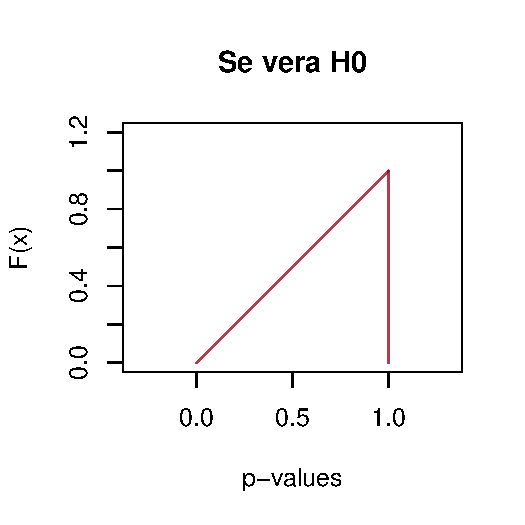
\includegraphics[width=0.3\textwidth]{plaatjes/cdf_uniform}      
     \end{center}
% \end{column}
% \end{columns}

\end{frame}


%%%%%%%%%%%%%%%%
\bfr{Errori di Tipo I:}%

\begin{overprint}
\only<1> {Sotto $H_0$ il p-value \`e una variabile aleatoria uniforme $U(0,1)$}
\only<2> {Errore di I tipo: $P(p\leq .05 |H_0)=.05$} % (o almeno $\leq .05$)}
\end{overprint} 
\begin{overprint} 
\onslide<1> \centerline{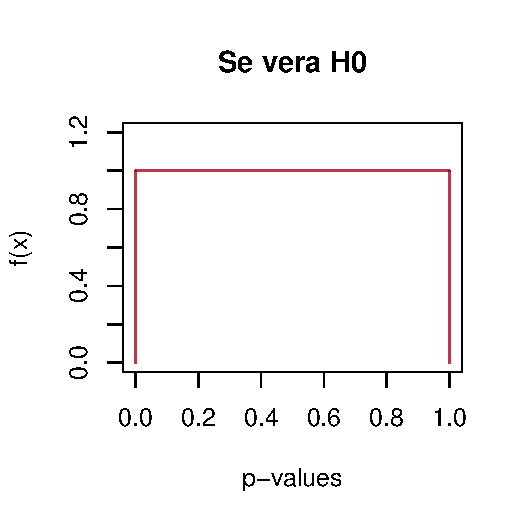
\includegraphics[width=8cm]{plaatjes/uniform1}}
\onslide<2> \centerline{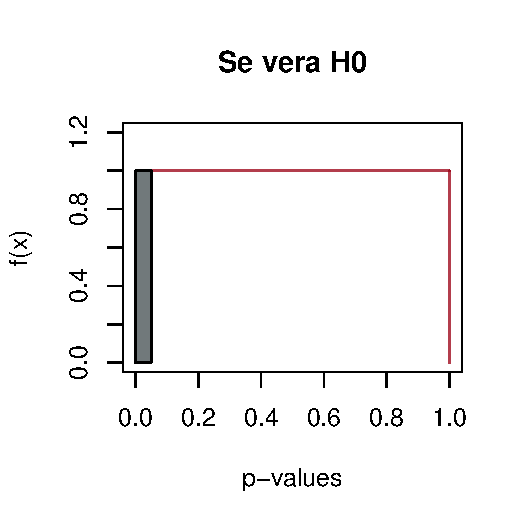
\includegraphics[width=8cm]{plaatjes/uniform2}}
\end{overprint} 
\end{frame}


\bfr{Potenza: $P(p\leq .05 | H_1=2\ gruppi\ Diversi)$}%
\begin{overprint}
% \onslide<7> ad es: $Potenza: P(p\leq 0.05 | H_1)=0.74$
\only<1> {\small Sotto $H_1$ il p-value \`e stocasticamente inferiore ad una variabile aleatoria uniforme $U(0,1)$ (Non distorsione del test)}
\onslide<2> {Sotto $H_1$ $P(p\leq .05 |H_1)>.05$, nel nostro caso $= .74$\\ }
\end{overprint}
\begin{overprint} 
\onslide<1> \centerline{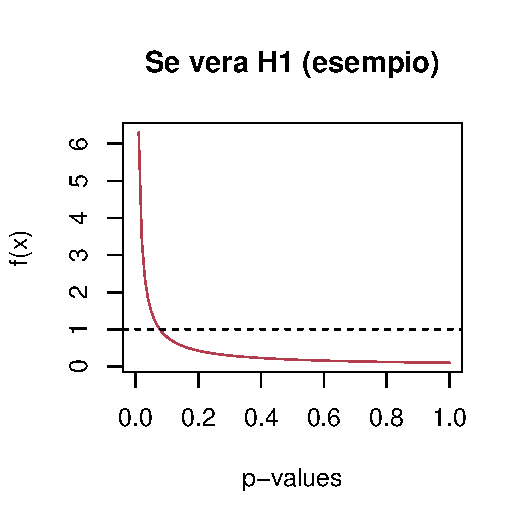
\includegraphics[width=7cm]{plaatjes/beta1}}
\onslide<2> \centerline{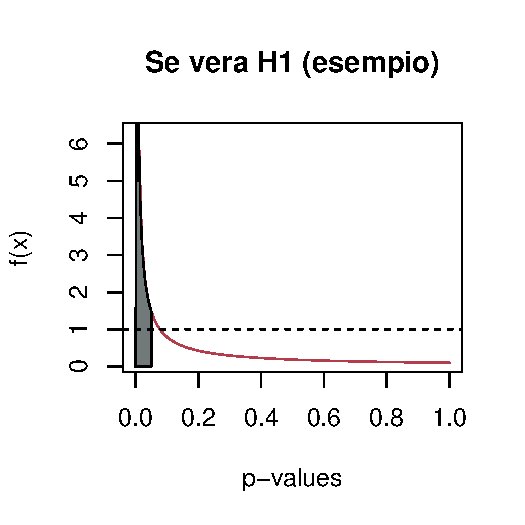
\includegraphics[width=7cm]{plaatjes/beta2}}
\end{overprint} 
\end{frame}


\bfr{Errori di Tipo I, Due Test (indipendenti)}%
Propabilit\`a di ALMENO un (falso) rifiuto?\\
  $P(p_1\leq .05 \cup p_2\leq .05 | H_0)= .05+.05-(.05\cdot .05)=1-(1-.05)^2=.0975=1-(1-\alpha)^2$

 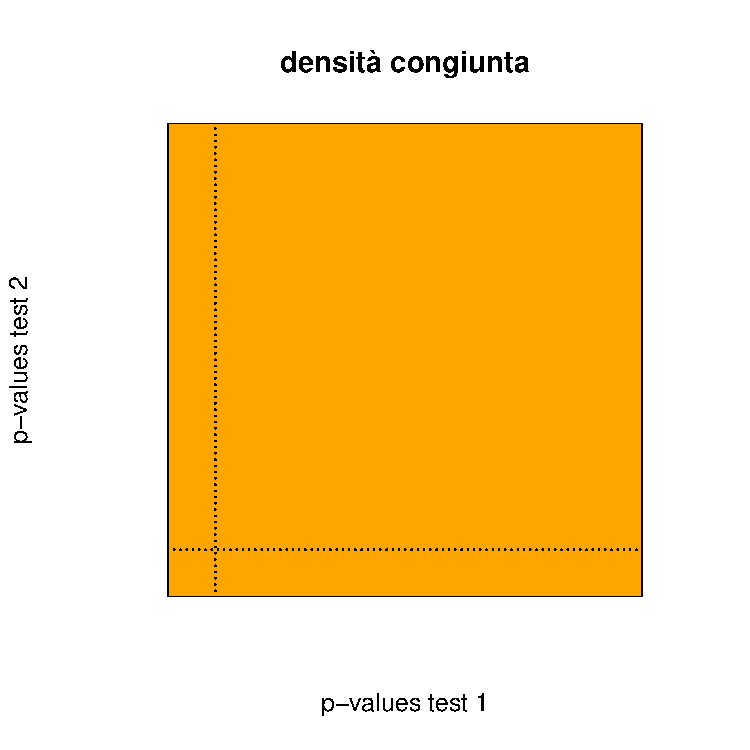
\includegraphics[scale=.5]{plaatjes/bivaH0indep}
\end{frame}

%\bfr{Potenza, Due Test}%
%\begin{overprint} 
%\onslide<1> 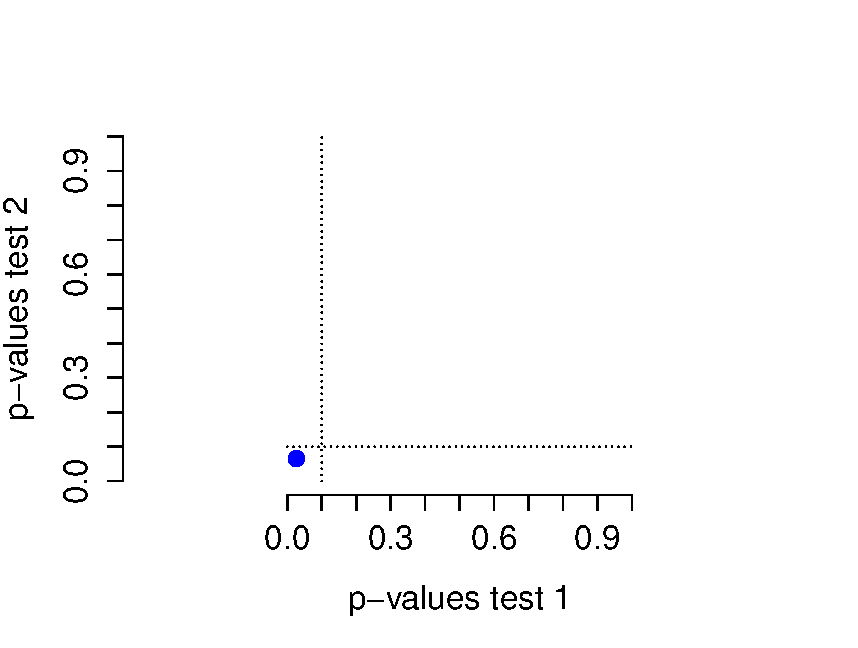
\includegraphics[scale=.5]{plaatjes/bivaH1_1}
%\onslide<2> 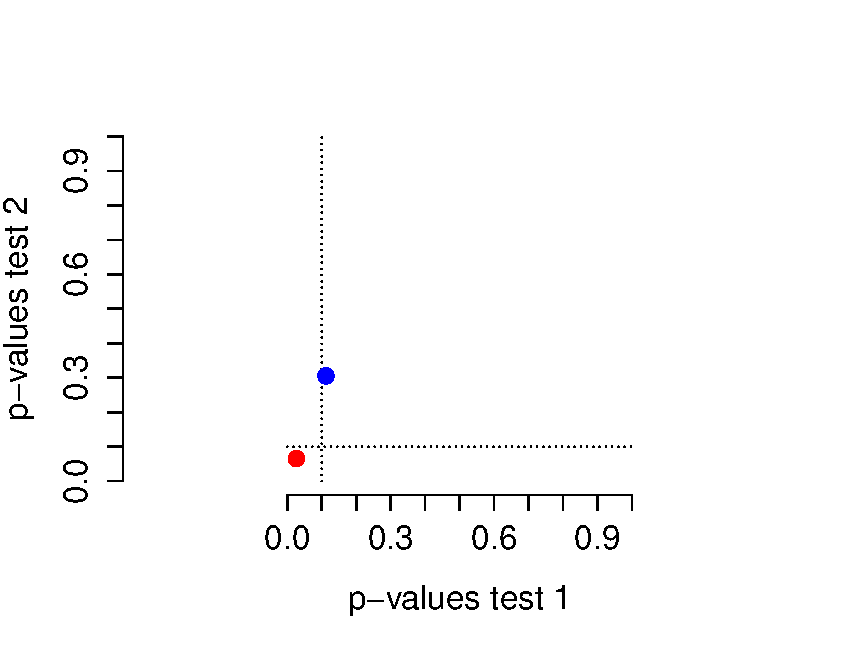
\includegraphics[scale=.5]{plaatjes/bivaH1_2}
%\onslide<3> 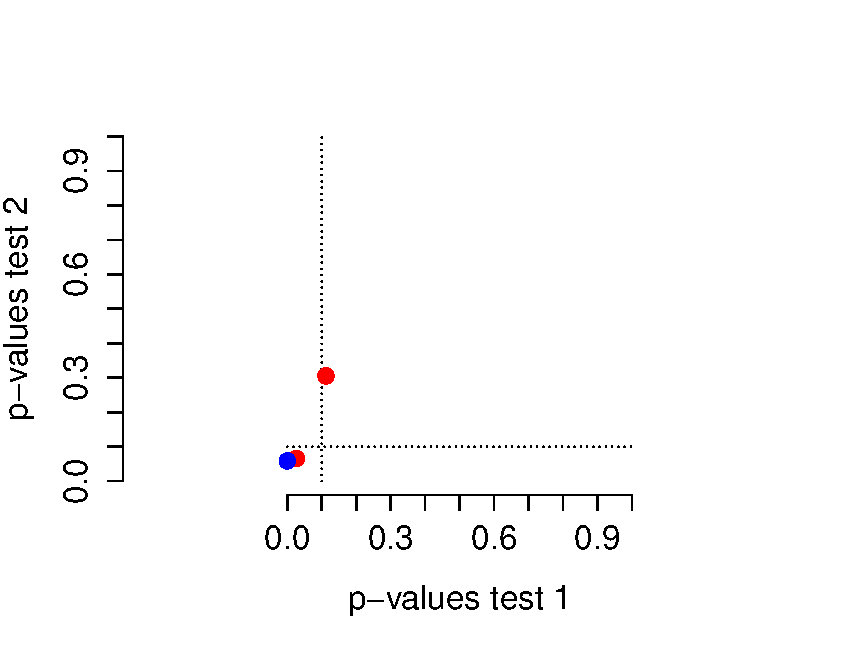
\includegraphics[scale=.5]{plaatjes/bivaH1_3}
%\onslide<4> 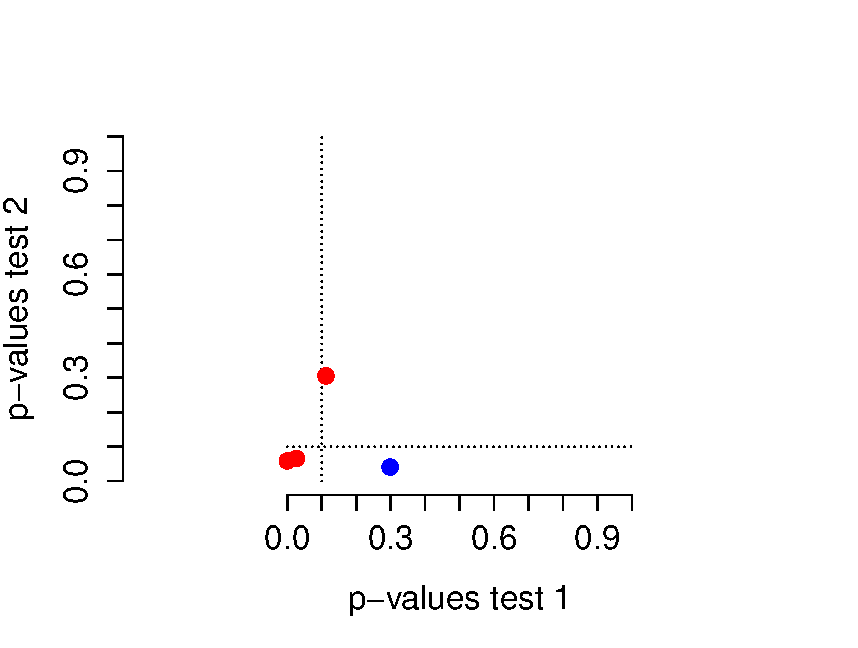
\includegraphics[scale=.5]{plaatjes/bivaH1_4}
%%\onslide<5> \includegraphics[scale=.5]{plaatjes/bivaH1_5}
%%\onslide<6> \includegraphics[scale=.5]{plaatjes/bivaH1_6}
%\onslide<5> 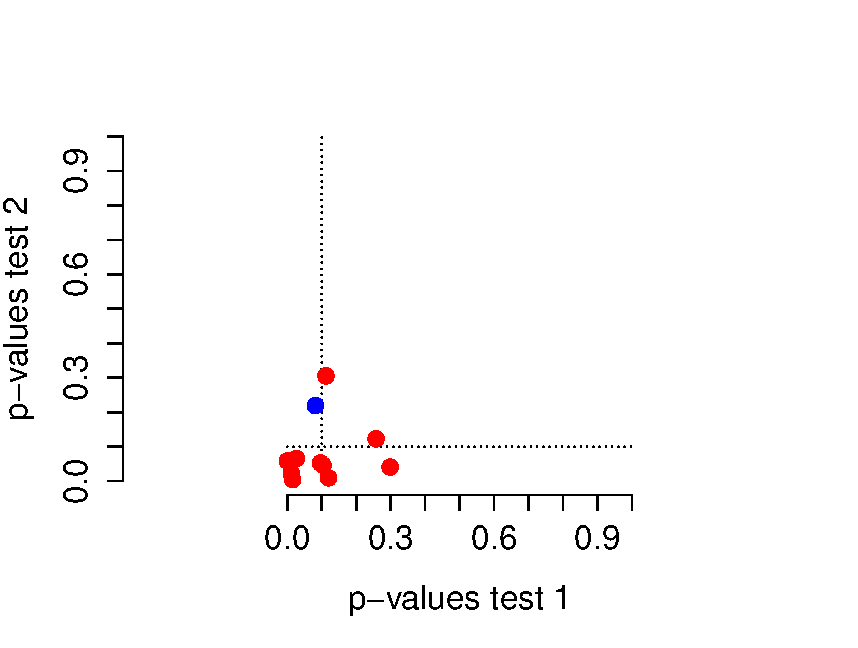
\includegraphics[scale=.5]{plaatjes/bivaH1_7}
%\onslide<6> 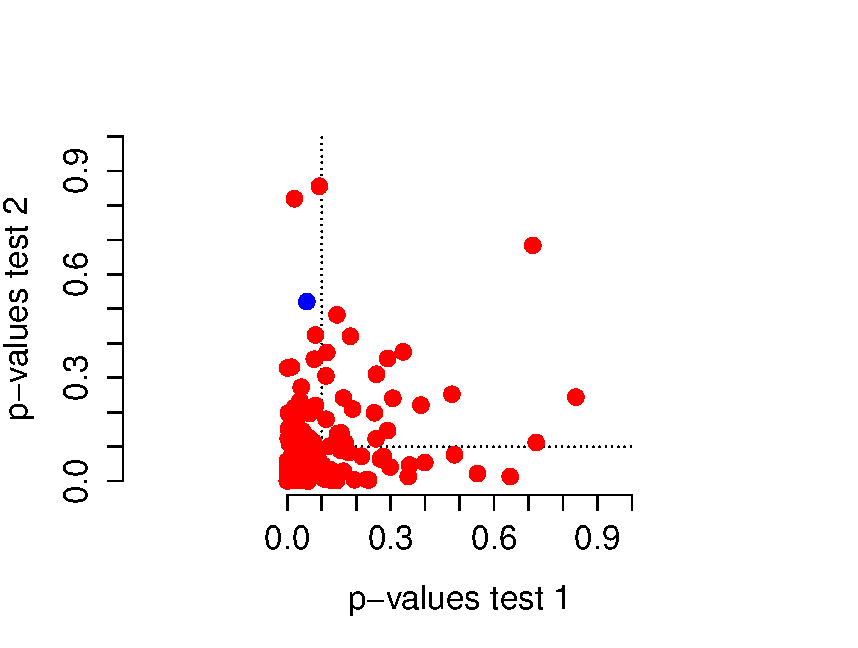
\includegraphics[scale=.5]{plaatjes/bivaH1_8}
%\onslide<7> 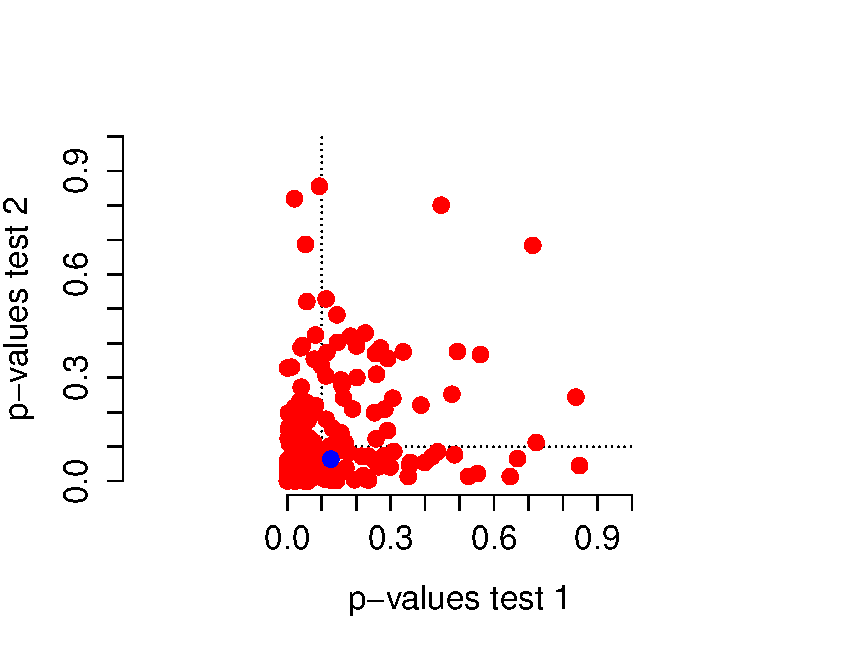
\includegraphics[scale=.5]{plaatjes/bivaH1_9}
%\end{overprint} 
%\end{frame}

\bfr{Probabilit\`a di falsi rifiuti}
  \bb{$m$ p-value indipendenti}
    Se rifiuto l'ipotesi quando $p\leq \alpha$
  \eb
  \bb{Probabilit\`a ALMENO un falso rifiuto}
    $P = 1- (1-\alpha)^m$
  \eb
  
  \pause
  \bigskip
Questo diventa ben presto un problema, se $m$ diventa grande ...

\end{frame}

\bfr{Errori di Tipo I in funzione del numero di test ($m$)}%
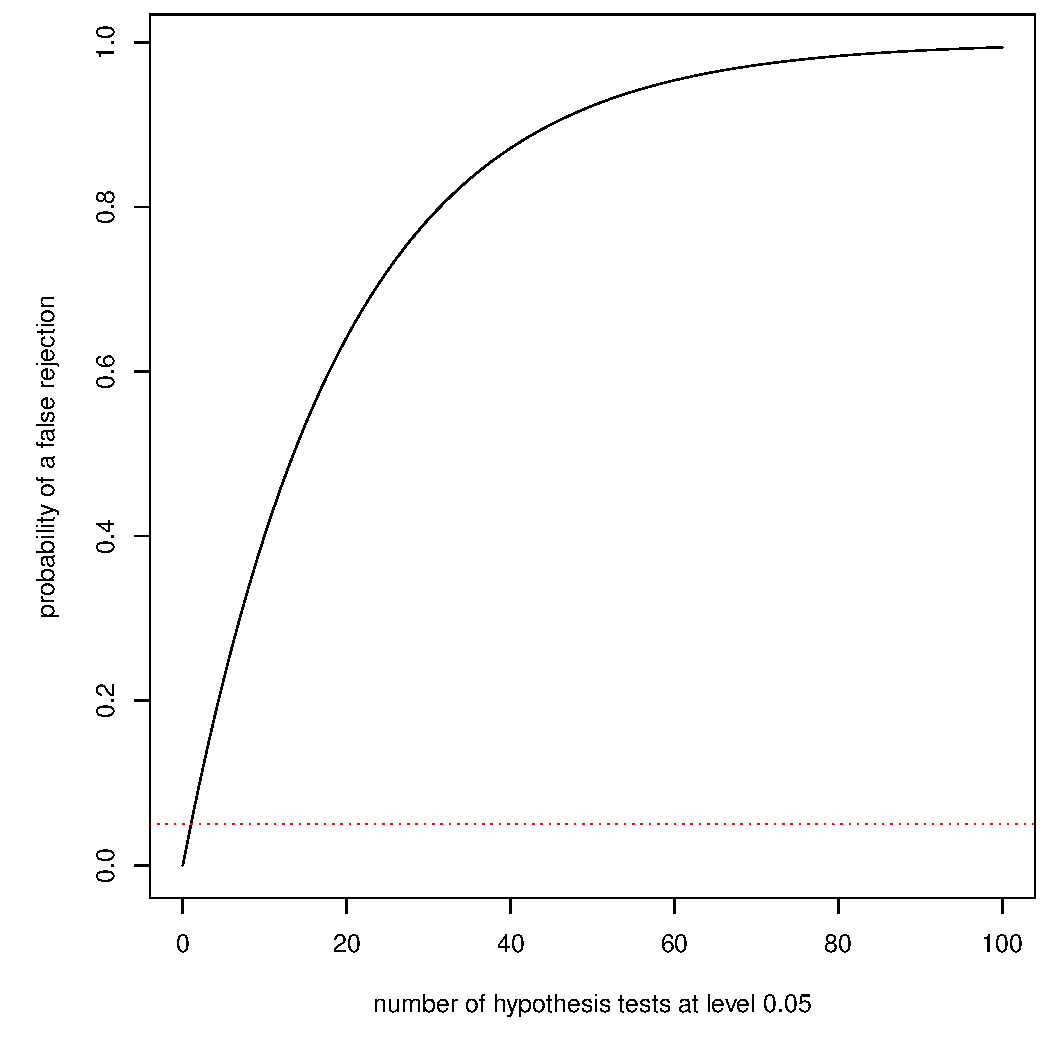
\includegraphics[scale=.3]{plaatjes/typeI}
\end{frame}

%\begin{frame}
%\frametitle{La Molteplicit\`a}
%Un test statistico produce un p-value ($0 < p \leq 1$). Caratteristiche:
%\begin{itemize}
%\item Se è vera $H_0$: $p\leq 0.05$ nel $5\%$ dei casi (errore di primo tipo, false discovery)
%\item Se è vera $H_1$: $p\leq 0.05$ con alta probabilt\`a, pi\`u del 5\% dei casi (potenza, veri rifiuti).
%\end{itemize}
%\bigskip
%Con {\bf un solo test} il controllo della probabilit\`a di errore del primo tipo è assicurato.\\
%\bigskip
%Cosa riusciamo ad garantire quando i test sono {\bf molti}? un esempio..
%\end{frame}
%%%%%%%%%%%%%%%%%%%%%%%%
%\subsection{}
%\begin{frame}
%\frametitle{Analogia tra test e dadi}

%Assumiamo (solo per questo esempio):
%\begin{itemize}
%\item tutti i test sotto l'{\bf ipotesi nulla} (femmine e maschi sono uguali) 
%\item gli item sono statisticamente indipendenti.  
%\item significativit\`a $\alpha=1/6=0.1667$ (rifiuto se $p<0.1667$)
%\end{itemize}
%\medskip
%Il risultato di un singolo test è assimilabile al lancio un dado:\\
%\begin{center}
%Probabilit\`a di rifiutare la {\bf singola ipotesi} (1 item) =\\
%= Probabilit\`a di $p\leq \alpha$ =\\
%= Probabilit\`a di fare \epsdice{1}\\
%\end{center}
% 
%\bigskip
%Controllare la {\bf molteplicit\`a} significa calcolare la probabilit\`a di fare ALMENO un \epsdice{1}\   negli 86 lanci (test riferiti agli item e scale):
%\begin{center}
%Probabilit\`a di fare ALMENO un  \epsdice{1}\ su 102 lanci = 1 !!\\
%\end{center}

%\end{frame}


\bfr{Type I errors}
    \bb{Come definire l'errore di tipo I quando ci sono molte ipotesi?}
\eb
       \bb{Quali procedure controllano questo errore?}
\eb
\end{frame}



%\section{Bonferroni, Holm and Shaffer}
%\subsection{Single step (Bonferroni)}


\end{document}


